\subsection{Turing Test}
The Turing test is a qualitative metric based on human perceptions. Due to our limited resources we just elaborate a short survey on Google Forms, divided into two sections: we asked the participants to first evaluate the colorizations of three black and white photographs and then evaluate the ri-colorizations of four originally colored images. 

A preliminary test has been conducted on few partecipants, who were always be able to dicriminate between the original version of the images and the ri-colorizations. Therefore, we decided to not show the original colored images in the final Turing test in order to avoid biases on the different and equally plausible choices of colors. 

The 124 participants had to score how realistic was each colorization in a
scale from 1 (not realistic at all) to 5 (very realistic). The test includes only the best colorizers, namely Eccv16, Siggraph17, ChromaGAN and InstColorization. 

Figure \ref{fig:turing} summarizes the mean scores for each model. Clearly, the models performed differently on originally colored images and greyscale photographs, since these ones have a low-level image statistics which are quite different from those of the modern-day photos on which the models were trained \cite{zhang}.
Overall, the best average scores are reached by Siggraph17 and ChromaGAN.

\begin{figure}[h]
	\centering
	\captionsetup[subfigure]{labelformat=empty}
	\begin{subfigure}[b]{0.1\textwidth}
		\begin{adjustwidth}{-1.1cm}{}
		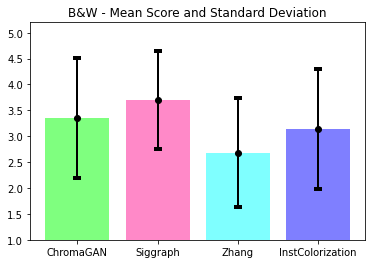
\includegraphics[width=4cm]{bw turing.png}
		\end{adjustwidth}
	\caption{B\&W}
	\end{subfigure}
\hspace{2.3cm}
	\begin{subfigure}[b]{0.1\textwidth}
		\begin{adjustwidth}{-1.1cm}{}
			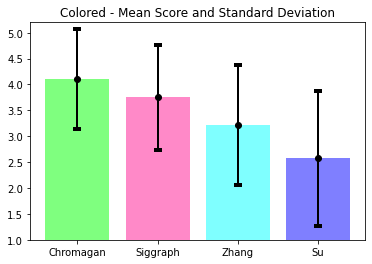
\includegraphics[width=4cm]{col turing.png}
		\end{adjustwidth}
		\caption{Colored}
	\end{subfigure}
	\caption{{\small Mean scores obtained with the colorization on black and white photographs and originally colored images.}}
	\label{fig:turing}
\end{figure}